\section{Background}
We provide brief introduction to capsule networks and convolutional networks in deep learning in context of graph theory.

\paragraph{Covolutional Neural Networks}
Convolutional Neural Networks (ConvNets or CNNs) are a category of Neural Networks that have proven very effective in areas such as image recognition and classification.
\begin{figure}[!htbp]
  \centering
  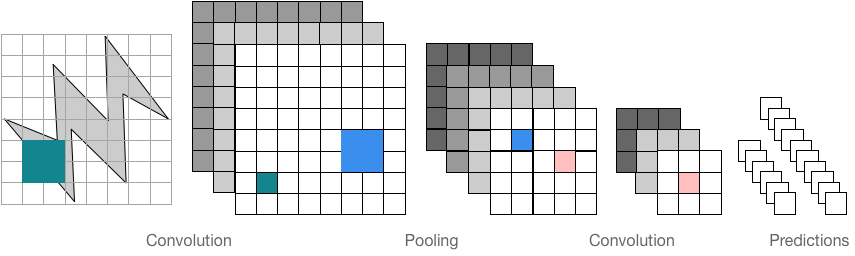
\includegraphics[width=\linewidth,height=\textheight,keepaspectratio]{images/CNN.png}
  \caption{CNN}
  \label{cnn}
\end{figure}
\FloatBarrier
Basic building blocks of Convolutional Neural Network are Convolution, Non Linearity (ReLU), Pooling or and Classification. When CNNs are used to classify images, a grid is move over each image with a particular step size. The receptive field reads the feature values for each channel in specific spatial order. The spatial order uniquely determines nodes of each receptive field and the way these nodes are mapped to a vector space representation. The values read from two pixels using two locations of receptive fields are assigned to the same relative position if and only if the pixels' structural roles are identical.

\paragraph{Capsule Network}
Convolutional neural networks work very well in various deep learning tasks but it has fundamental drawback. Simple example is rotated image \ref{k}. Orientational and relative spatial relationships between components are less important in CNN sicne higher-level features combine lower level features as a weighted sum that is sum of activations of preceding layers multiplied by weights. In this process relationshipe between simpler features are lost that make up higher level feature. To solve this problem CNNs use max pooling or successive layers to reduce spacial size of the data flowing through the network. Although, max pooling works well, it looses spatial information on features.
Capsule is a group of neurons whose activity represents the instantiation parameters of entities. The length of the activity vector represents the probability that the entity exists and its orientation to represent the instantiation parameters. In Caps net allows to keep relative relationship between objects which is represented as multi dimentional matrix.

\begin{figure}[!htbp]
  \centering
  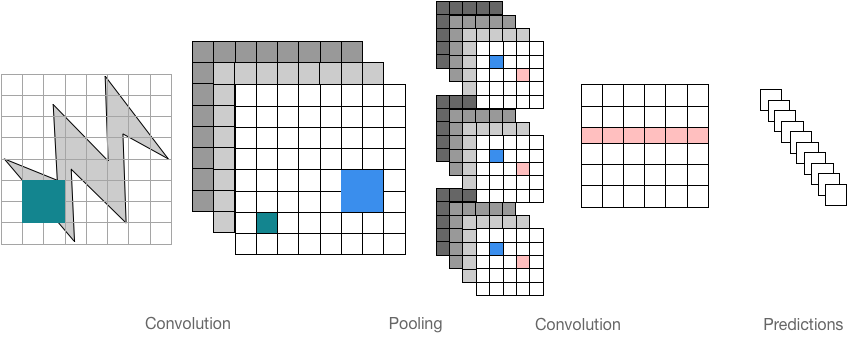
\includegraphics[width=\linewidth,height=\textheight,keepaspectratio]{images/CapsNet.png}
  \caption{Capsule Network Architecture}
  \label{k}
\end{figure}
\FloatBarrier
